\section{Feliratok kezelése}
A feliratok megjelenítése az alkalmazás magját alkotó funkciók közé sorolható, hiszen enélkül maga a nyelvtanulási folyamat nehezen lenne megvalósítható. Tehát e lehetőség használhatósága kulcsfontosságú a projekt tekintetében. Ennek a működését, implementálását bemutató fejezet logikailag két részre osztható: az \textit{.srt} kiterjesztésű fájlok beolvasása, kezelése, illetve a feliratok képernyőre történő kirajzolása.

\subsection{Feliratfájlok beolvasása}
Ahhoz, hogy a szoftver képes legyen feliratokat megjeleníteni, tudnia kell azokat a felhasználó számítógépéről felolvasni, kezelni. Az alkalmazás jelenleg csak a \textit{SubRip}, azaz \textit{.srt} kiterjesztésű fájlok kezelését támogatja, mivel az említett formátum a legelterjedtebb típusok közé sorolható. Előállításuk, interneten való fellelésük rendkívül könnyű, gyors, emiatt nagy népszerűségnek örvend mind a felirat elkészítői, mind a felirat használói közt. Strukturális felépítése egyszerű, a \ref{lst:srt} ábrán látható.


\todo[inline]{Legyen lst listing ez is}
\begin{verbatim}
1
00:00:01,100 --> 00:00:01,500
First line
Second line
 
2 
00:00:25,0004 --> 00:00:30,200 
Additional text...
\end{verbatim}

A fájl blokkokra osztható, amelyek egy-egy megjelenítendő feliratrészletnek felelnek meg. Minden ilyen rész első sorában egy sorszám található. Ezek a részletek azonosítására szolgálnak. A következő sorban a kezdő-, illetve a végidőpontok helyezkednek el, közöttük egy szigorúan „-->” alakú nyíllal, előtte és utána szóközökkel határolva. Az időpontokat konvenció szerint óra:perc:másodperc,ezredmásodperc formátumban kötelező megadni. Ezután a vászonra kirajzolandó sorok találhatóak. Itt fontos megemlíteni, hogy a fájl érzékeny a sortörésekre, hiszen ezek alapján tesz különbséget a más-más sorokba kerülő szövegek között. A szöveg sora(i) után legalább egy üres sornak kell szerepelnie. Amennyiben ez hiányzik, a következő blokk az előző szövegrészébe kerül.
A feliratfájlok kezeléséért az \textit{srt} package-ben található \textit{Java} osztályok felelősek. A fő funkcionalitásokat, azaz a feliratok beolvasását, feldolgozását az \textit{SRTReader.java} nevű osztály végzi az itt található \textit{read}, illetve \textit{parse} metódusok segítségével. Az előbbi egy \textit{File} objektumot vár, amit a soronként dolgoz fel, és minden soron alkalmazza a \textit{parse} metódust, ami egy \textit{TreeSet}-hez adja hozzá a feldolgozott blokkoknak megfelelő \textit{Java} objektumokat (\ref{lst:srt_feldolgozas}).

\begin{lstlisting}[caption=Srt fájlok feldolgozása, label={lst:srt_feldolgozas}, language=java]
public static SRTInfo read(File srtFile) 
throws InvalidSRTException, SRTReaderException {
    if (!srtFile.exists()) {
        throw new SRTReaderException(srtFile.getAbsolutePath()
        + " does not exist");
    }
    if (!srtFile.isFile()) {
        throw new SRTReaderException(srtFile.getAbsolutePath()
        + " is not a regular file");
    }

    SRTInfo srtInfo = new SRTInfo();
    try (BufferedReader br = new BufferedReader
    (new InputStreamReader(
            new FileInputStream(srtFile),
            StandardCharsets.UTF_8))) {
        BufferedLineReader reader = new BufferedLineReader(br);
        while (true) {
            srtInfo.add(parse(reader));
        }
    } catch (EOFException e) {
    } catch (IOException e) {
        throw new SRTReaderException(e);
    }
    
    return srtInfo;
}
\end{lstlisting}

  A függvény képes kivételek kezelésére is. Amennyiben az átadott fájl nem létezik, például végrehajtás közben törölték, illetve, ha a fájl nem reguláris fájl, azaz nem fájlrendszerben tárolt bájtok sorozata, az alkalmazás erről megfelelő hibaüzenetet továbbít.
  
\subsection{Feliratok megjelenítése}
Mivel a feliratokat tartalmazó fájlokat az alkalmazás már be tudja olvasni, valamint képes azok kezelésére, a soron következő megvalósítandó funkció ezen feliratok képernyőn történő megjelenítése, olyan módon, ahogyan az egy általános videólejátszó szoftvertől elvárható. Fontos szempont tehát az időzítés, illetve a feliratok megfelelő formátumú kirajzolása. Ezen felül követelmény az is, hogy a megjelenő feliratokra kattintva láthatóak legyen az elérhető fordítások is. Ugyan a \textit{vlcj} függvénykönyvtárában található metódus, amely a feliratfájlok beállítását végzi, de mivel e funkció implementációja teljesen rejtett a \textit{Java}-s környezet elől, így nem volt arra lehetőség, hogy az egyes kirajzolt mondatrészekhez olyan figyelőt rendeljek, amely az egér kattintásait elemzi. Emiatt saját felirat megjelenítő komponenst kellett létrehozni, ami segítségével kattintásra elkérhető a szóból alkotott \textit{String} objektum, így majd a fordítás is megvalósulhat. A funkcióért a \textit{SubtitleOverlay} osztály felelős, amely elkészíti a megjelenítendő szöveget, és ki is rajzolja azt. Az osztály őse egy \textit{AWT} komponens, egy \textit{Window}, amely egy láthatatlan rétegként kerül a szoftver felhasználói felületére. Egyetlen feladata, a feliratok megjelenítése, pozicionálása, interakció megvalósítása. A felirat megjelenítésének megvalósítását a \textit{paint} függvény hajtja végre, amely a \ref{lst:felirat_megj} ábrán látható.

\begin{lstlisting}[caption=A felirat megjelenítése, language=java, label={lst:felirat_megj}]
@Override
public void paint(Graphics g) {
   super.paint(g);

   g.clearRect(0, 0, this.getWidth(), this.getHeight());

   Graphics2D g2 = (Graphics2D) g;
   g2.setRenderingHint(RenderingHints.KEY_ANTIALIASING,
   RenderingHints.VALUE_ANTIALIAS_ON);

   g2.setFont(new Font("Serif", Font.PLAIN, fontSize));
   g2.setColor(new Color(255, 255, 255));

   if(actSubtitle == null) {
      return;
   }
   
   calculateSubtitleBoundingBox(g2, actSubtitle);

   for (Entry<String, Rectangle2D> box : boundingBoxes) {
      g2.drawString(box.getKey(),
      (int)box.getValue().getX(),
      (int)(box.getValue().getY()+box.getValue().getHeight()));
   }
}
\end{lstlisting}

A kattintásra történő szöveg visszaadásának megvalósítása az egyes szavakat befoglaló kattintható, láthatatlan téglalapok segítségével történik. Az antialiasing, betűtípus, valamint a betűszín beállítása után a meghívott \textit{calculateSubtitleBoundingBox} végzi el a mondatelemek köré szánt négyszögek kiszámítását. A szavak, valamint az őket körül vevő téglalapok egy kulcs-érték párokat tároló Map-be kerülnek. A map elemeit alkalmazás a kattintás pozíciójának vizsgálatakor elemzi, és amennyiben a kattintás valamely map-ben fellelhető négyszög területén belülre esik, a szoftver visszaadja a hozzá tartozó kulcsot, jelen esetben a \textit{String} objektumot, amely a kattintott mondatelemet tartalmazza. Így tehát lehetőség nyílik a felhasználó egérrel történő kattintásait nyomon követni, és ennek megfelelően elvégezni a szükséges fordítást. A kód minimális módosításával megjeleníthetők a befoglaló téglalapok, így jól látható, hogy a szoftver mely területekre figyel a felhasználó kattintásai során.
\begin{figure}
  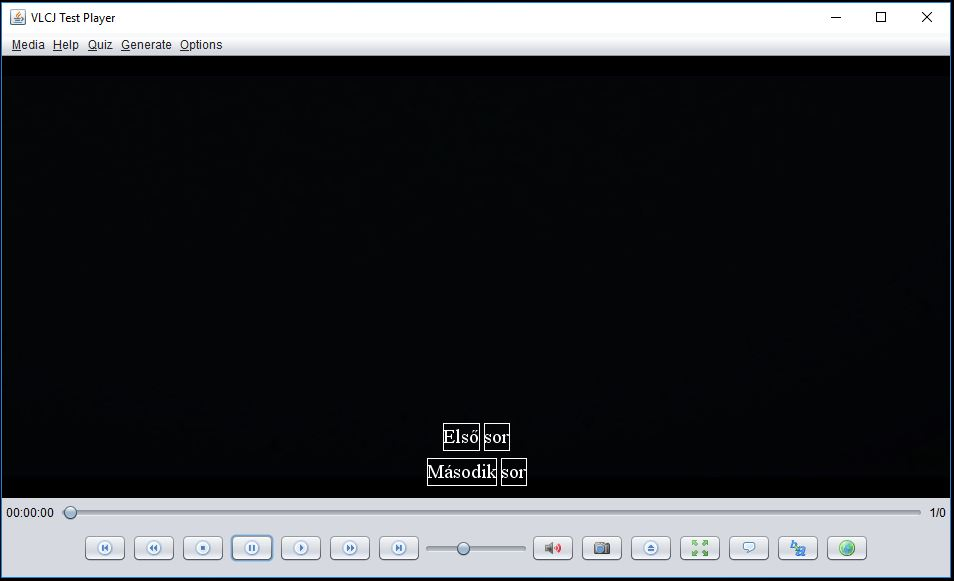
\includegraphics[width=\linewidth]{images/subtitle_boxes.jpg}
  \caption{A befoglaló négyszögek megjelenítve a szavak körül}
  \label{fig:full_screen}
\end{figure}
A bemutatott két funkció alkalmazásba történő implementálásával lehetőség nyílt arra, hogy a felhasználó interakcióit a szoftver dinamikusan, a film lejátszása közben kezelje, illetve ennek alapján megfelelő fordításokat végezzen beépített fordító API segítségével.
